\documentclass[1p]{elsarticle_modified}
%\bibliographystyle{elsarticle-num}

%\usepackage[colorlinks]{hyperref}
%\usepackage{abbrmath_seonhwa} %\Abb, \Ascr, \Acal ,\Abf, \Afrak
\usepackage{amsfonts}
\usepackage{amssymb}
\usepackage{amsmath}
\usepackage{amsthm}
\usepackage{scalefnt}
\usepackage{amsbsy}
\usepackage{kotex}
\usepackage{caption}
\usepackage{subfig}
\usepackage{color}
\usepackage{graphicx}
\usepackage{xcolor} %% white, black, red, green, blue, cyan, magenta, yellow
\usepackage{float}
\usepackage{setspace}
\usepackage{hyperref}

\usepackage{tikz}
\usetikzlibrary{arrows}

\usepackage{multirow}
\usepackage{array} % fixed length table
\usepackage{hhline}

%%%%%%%%%%%%%%%%%%%%%
\makeatletter
\renewcommand*\env@matrix[1][\arraystretch]{%
	\edef\arraystretch{#1}%
	\hskip -\arraycolsep
	\let\@ifnextchar\new@ifnextchar
	\array{*\c@MaxMatrixCols c}}
\makeatother %https://tex.stackexchange.com/questions/14071/how-can-i-increase-the-line-spacing-in-a-matrix
%%%%%%%%%%%%%%%

\usepackage[normalem]{ulem}

\newcommand{\msout}[1]{\ifmmode\text{\sout{\ensuremath{#1}}}\else\sout{#1}\fi}
%SOURCE: \msout is \stkout macro in https://tex.stackexchange.com/questions/20609/strikeout-in-math-mode

\newcommand{\cancel}[1]{
	\ifmmode
	{\color{red}\msout{#1}}
	\else
	{\color{red}\sout{#1}}
	\fi
}

\newcommand{\add}[1]{
	{\color{blue}\uwave{#1}}
}

\newcommand{\replace}[2]{
	\ifmmode
	{\color{red}\msout{#1}}{\color{blue}\uwave{#2}}
	\else
	{\color{red}\sout{#1}}{\color{blue}\uwave{#2}}
	\fi
}

\newcommand{\Sol}{\mathcal{S}} %segment
\newcommand{\D}{D} %diagram
\newcommand{\A}{\mathcal{A}} %arc


%%%%%%%%%%%%%%%%%%%%%%%%%%%%%5 test

\def\sl{\operatorname{\textup{SL}}(2,\Cbb)}
\def\psl{\operatorname{\textup{PSL}}(2,\Cbb)}
\def\quan{\mkern 1mu \triangleright \mkern 1mu}

\theoremstyle{definition}
\newtheorem{thm}{Theorem}[section]
\newtheorem{prop}[thm]{Proposition}
\newtheorem{lem}[thm]{Lemma}
\newtheorem{ques}[thm]{Question}
\newtheorem{cor}[thm]{Corollary}
\newtheorem{defn}[thm]{Definition}
\newtheorem{exam}[thm]{Example}
\newtheorem{rmk}[thm]{Remark}
\newtheorem{alg}[thm]{Algorithm}

\newcommand{\I}{\sqrt{-1}}
\begin{document}

%\begin{frontmatter}
%
%\title{Boundary parabolic representations of knots up to 8 crossings}
%
%%% Group authors per affiliation:
%\author{Yunhi Cho} 
%\address{Department of Mathematics, University of Seoul, Seoul, Korea}
%\ead{yhcho@uos.ac.kr}
%
%
%\author{Seonhwa Kim} %\fnref{s_kim}}
%\address{Center for Geometry and Physics, Institute for Basic Science, Pohang, 37673, Korea}
%\ead{ryeona17@ibs.re.kr}
%
%\author{Hyuk Kim}
%\address{Department of Mathematical Sciences, Seoul National University, Seoul 08826, Korea}
%\ead{hyukkim@snu.ac.kr}
%
%\author{Seokbeom Yoon}
%\address{Department of Mathematical Sciences, Seoul National University, Seoul, 08826,  Korea}
%\ead{sbyoon15@snu.ac.kr}
%
%\begin{abstract}
%We find all boundary parabolic representation of knots up to 8 crossings.
%
%\end{abstract}
%\begin{keyword}
%    \MSC[2010] 57M25 
%\end{keyword}
%
%\end{frontmatter}

%\linenumbers
%\tableofcontents
%
\newcommand\colored[1]{\textcolor{white}{\rule[-0.35ex]{0.8em}{1.4ex}}\kern-0.8em\color{red} #1}%
%\newcommand\colored[1]{\textcolor{white}{ #1}\kern-2.17ex	\textcolor{white}{ #1}\kern-1.81ex	\textcolor{white}{ #1}\kern-2.15ex\color{red}#1	}

{\Large $\underline{12n_{0735}~(K12n_{0735})}$}

\setlength{\tabcolsep}{10pt}
\renewcommand{\arraystretch}{1.6}
\vspace{1cm}\begin{tabular}{m{100pt}>{\centering\arraybackslash}m{274pt}}
\multirow{5}{120pt}{
	\centering
	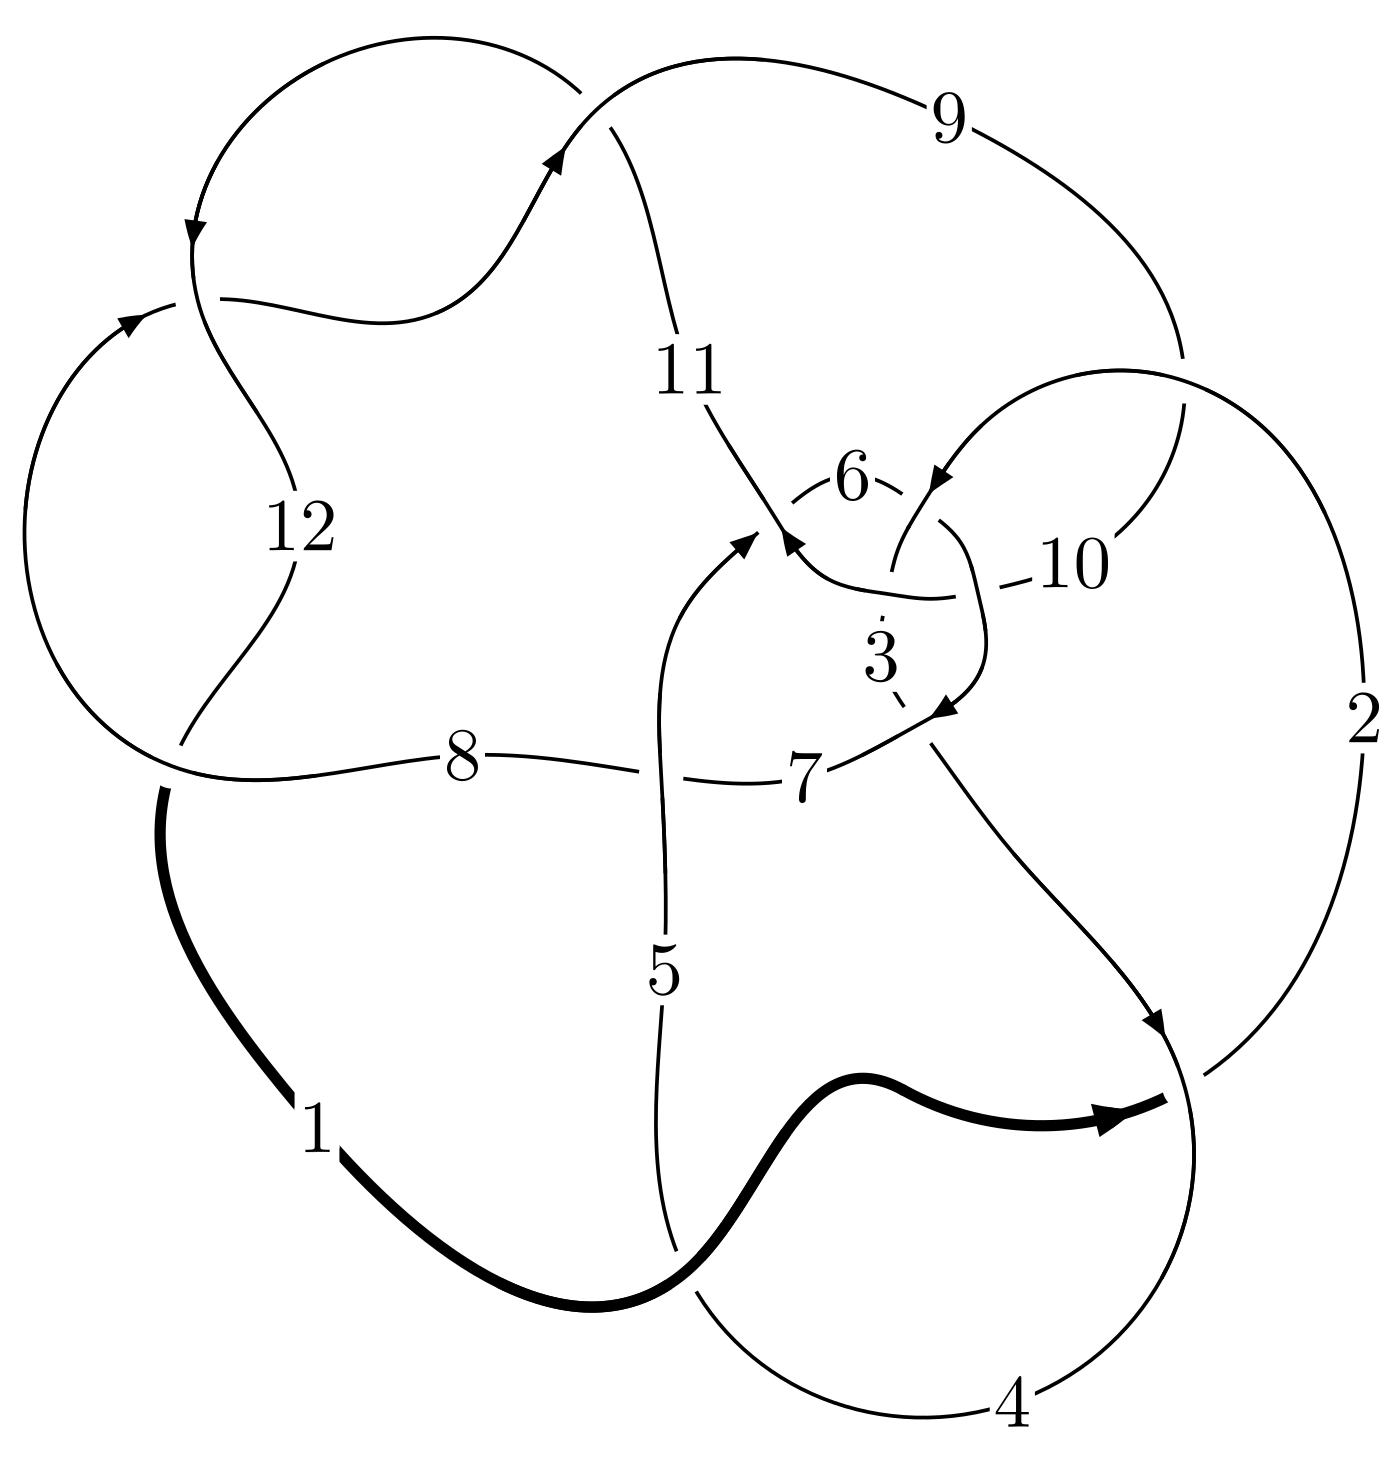
\includegraphics[width=112pt]{../../../GIT/diagram.site/Diagrams/png/2824_12n_0735.png}\\
\ \ \ A knot diagram\footnotemark}&
\allowdisplaybreaks
\textbf{Linearized knot diagam} \\
\cline{2-2}
 &
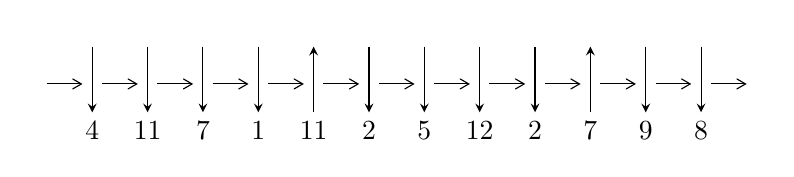
\begin{tikzpicture}[x=20pt, y=17pt]
	% nodes
	\node (C0) at (0, 0) {};
	\node (C1) at (1, 0) {};
	\node (C1U) at (1, +1) {};
	\node (C1D) at (1, -1) {4};

	\node (C2) at (2, 0) {};
	\node (C2U) at (2, +1) {};
	\node (C2D) at (2, -1) {11};

	\node (C3) at (3, 0) {};
	\node (C3U) at (3, +1) {};
	\node (C3D) at (3, -1) {7};

	\node (C4) at (4, 0) {};
	\node (C4U) at (4, +1) {};
	\node (C4D) at (4, -1) {1};

	\node (C5) at (5, 0) {};
	\node (C5U) at (5, +1) {};
	\node (C5D) at (5, -1) {11};

	\node (C6) at (6, 0) {};
	\node (C6U) at (6, +1) {};
	\node (C6D) at (6, -1) {2};

	\node (C7) at (7, 0) {};
	\node (C7U) at (7, +1) {};
	\node (C7D) at (7, -1) {5};

	\node (C8) at (8, 0) {};
	\node (C8U) at (8, +1) {};
	\node (C8D) at (8, -1) {12};

	\node (C9) at (9, 0) {};
	\node (C9U) at (9, +1) {};
	\node (C9D) at (9, -1) {2};

	\node (C10) at (10, 0) {};
	\node (C10U) at (10, +1) {};
	\node (C10D) at (10, -1) {7};

	\node (C11) at (11, 0) {};
	\node (C11U) at (11, +1) {};
	\node (C11D) at (11, -1) {9};

	\node (C12) at (12, 0) {};
	\node (C12U) at (12, +1) {};
	\node (C12D) at (12, -1) {8};
	\node (C13) at (13, 0) {};

	% arrows
	\draw[->,>={angle 60}]
	(C0) edge (C1) (C1) edge (C2) (C2) edge (C3) (C3) edge (C4) (C4) edge (C5) (C5) edge (C6) (C6) edge (C7) (C7) edge (C8) (C8) edge (C9) (C9) edge (C10) (C10) edge (C11) (C11) edge (C12) (C12) edge (C13) ;	\draw[->,>=stealth]
	(C1U) edge (C1D) (C2U) edge (C2D) (C3U) edge (C3D) (C4U) edge (C4D) (C5D) edge (C5U) (C6U) edge (C6D) (C7U) edge (C7D) (C8U) edge (C8D) (C9U) edge (C9D) (C10D) edge (C10U) (C11U) edge (C11D) (C12U) edge (C12D) ;
	\end{tikzpicture} \\
\hhline{~~} \\& 
\textbf{Solving Sequence} \\ \cline{2-2} 
 &
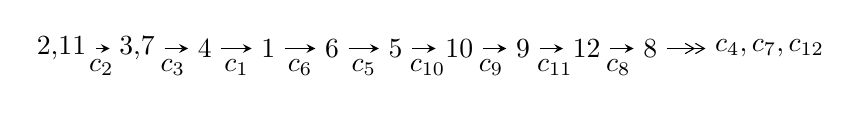
\begin{tikzpicture}[x=23pt, y=7pt]
	% node
	\node (A0) at (-1/8, 0) {2,11};
	\node (A1) at (17/16, 0) {3,7};
	\node (A2) at (17/8, 0) {4};
	\node (A3) at (25/8, 0) {1};
	\node (A4) at (33/8, 0) {6};
	\node (A5) at (41/8, 0) {5};
	\node (A6) at (49/8, 0) {10};
	\node (A7) at (57/8, 0) {9};
	\node (A8) at (65/8, 0) {12};
	\node (A9) at (73/8, 0) {8};
	\node (C1) at (1/2, -1) {$c_{2}$};
	\node (C2) at (13/8, -1) {$c_{3}$};
	\node (C3) at (21/8, -1) {$c_{1}$};
	\node (C4) at (29/8, -1) {$c_{6}$};
	\node (C5) at (37/8, -1) {$c_{5}$};
	\node (C6) at (45/8, -1) {$c_{10}$};
	\node (C7) at (53/8, -1) {$c_{9}$};
	\node (C8) at (61/8, -1) {$c_{11}$};
	\node (C9) at (69/8, -1) {$c_{8}$};
	\node (A10) at (11, 0) {$c_{4},c_{7},c_{12}$};

	% edge
	\draw[->,>=stealth]	
	(A0) edge (A1) (A1) edge (A2) (A2) edge (A3) (A3) edge (A4) (A4) edge (A5) (A5) edge (A6) (A6) edge (A7) (A7) edge (A8) (A8) edge (A9) ;
	\draw[->>,>={angle 60}]	
	(A9) edge (A10);
\end{tikzpicture} \\ 

\end{tabular} \\

\footnotetext{
The image of knot diagram is generated by the software ``\textbf{Draw programme}" developed by Andrew Bartholomew(\url{http://www.layer8.co.uk/maths/draw/index.htm\#Running-draw}), where we modified some parts for our purpose(\url{https://github.com/CATsTAILs/LinksPainter}).
}\phantom \\ \newline 
\centering \textbf{Ideals for irreducible components\footnotemark of $X_{\text{par}}$} 
 
\begin{align*}
I^u_{1}&=\langle 
1.47491\times10^{161} u^{52}-1.00334\times10^{161} u^{51}+\cdots+6.59902\times10^{163} b-4.00631\times10^{164},\\
\phantom{I^u_{1}}&\phantom{= \langle  }1.55727\times10^{164} u^{52}-4.68658\times10^{163} u^{51}+\cdots+6.14369\times10^{166} a-7.33068\times10^{167},\\
\phantom{I^u_{1}}&\phantom{= \langle  }u^{53}- u^{52}+\cdots+1260 u-931\rangle \\
I^u_{2}&=\langle 
-1092 u^{17}+1979 u^{16}+\cdots+1579 b-2918,\;-862 u^{17}-922 u^{16}+\cdots+1579 a+3868,\\
\phantom{I^u_{2}}&\phantom{= \langle  }u^{18}+6 u^{16}- u^{15}+10 u^{14}-4 u^{13}+2 u^{12}-4 u^{11}+u^{10}-4 u^9+5 u^8-5 u^7-4 u^6+6 u^5+8 u^4-3 u^3-4 u^2+1\rangle \\
\\
\end{align*}
\raggedright * 2 irreducible components of $\dim_{\mathbb{C}}=0$, with total 71 representations.\\
\footnotetext{All coefficients of polynomials are rational numbers. But the coefficients are sometimes approximated in decimal forms when there is not enough margin.}
\newpage
\renewcommand{\arraystretch}{1}
\centering \section*{I. $I^u_{1}= \langle 1.47\times10^{161} u^{52}-1.00\times10^{161} u^{51}+\cdots+6.60\times10^{163} b-4.01\times10^{164},\;1.56\times10^{164} u^{52}-4.69\times10^{163} u^{51}+\cdots+6.14\times10^{166} a-7.33\times10^{167},\;u^{53}- u^{52}+\cdots+1260 u-931 \rangle$}
\flushleft \textbf{(i) Arc colorings}\\
\begin{tabular}{m{7pt} m{180pt} m{7pt} m{180pt} }
\flushright $a_{2}=$&$\begin{pmatrix}1\\0\end{pmatrix}$ \\
\flushright $a_{11}=$&$\begin{pmatrix}0\\u\end{pmatrix}$ \\
\flushright $a_{3}=$&$\begin{pmatrix}1\\u^2\end{pmatrix}$ \\
\flushright $a_{7}=$&$\begin{pmatrix}-0.00253474 u^{52}+0.000762828 u^{51}+\cdots-12.6342 u+11.9320\\-0.00223505 u^{52}+0.00152044 u^{51}+\cdots-5.41272 u+6.07107\end{pmatrix}$ \\
\flushright $a_{4}=$&$\begin{pmatrix}0.000307309 u^{52}-0.00341411 u^{51}+\cdots-25.6189 u+13.2717\\0.00388609 u^{52}-0.00479985 u^{51}+\cdots-9.07382 u-1.92407\end{pmatrix}$ \\
\flushright $a_{1}=$&$\begin{pmatrix}0.000445713 u^{52}-0.00127751 u^{51}+\cdots-7.34876 u+4.21132\\0.000455151 u^{52}+0.00111184 u^{51}+\cdots+16.0717 u-6.35644\end{pmatrix}$ \\
\flushright $a_{6}=$&$\begin{pmatrix}-0.00476979 u^{52}+0.00228326 u^{51}+\cdots-18.0470 u+18.0031\\-0.00223505 u^{52}+0.00152044 u^{51}+\cdots-5.41272 u+6.07107\end{pmatrix}$ \\
\flushright $a_{5}=$&$\begin{pmatrix}-0.00476979 u^{52}+0.00228326 u^{51}+\cdots-18.0470 u+18.0031\\-0.000888908 u^{52}+0.000380323 u^{51}+\cdots-6.72037 u+3.75612\end{pmatrix}$ \\
\flushright $a_{10}=$&$\begin{pmatrix}0.00734689 u^{52}-0.00837266 u^{51}+\cdots-33.0209 u+0.0462951\\0.00168842 u^{52}-0.00168620 u^{51}+\cdots-2.75207 u-1.24109\end{pmatrix}$ \\
\flushright $a_{9}=$&$\begin{pmatrix}0.00903531 u^{52}-0.0100589 u^{51}+\cdots-35.7730 u-1.19480\\0.00168842 u^{52}-0.00168620 u^{51}+\cdots-2.75207 u-1.24109\end{pmatrix}$ \\
\flushright $a_{12}=$&$\begin{pmatrix}0.000777537 u^{52}-0.00530471 u^{51}+\cdots-33.5819 u+14.2472\\0.00375707 u^{52}-0.00500103 u^{51}+\cdots-18.9354 u+2.02528\end{pmatrix}$ \\
\flushright $a_{8}=$&$\begin{pmatrix}-0.00441879 u^{52}+0.00343811 u^{51}+\cdots-10.9752 u+9.12520\\0.00140540 u^{52}-0.00443957 u^{51}+\cdots-26.4019 u+9.54110\end{pmatrix}$\\&\end{tabular}
\flushleft \textbf{(ii) Obstruction class $= -1$}\\~\\
\flushleft \textbf{(iii) Cusp Shapes $= -0.00251009 u^{52}-0.00470979 u^{51}+\cdots+12.2699 u+11.1088$}\\~\\
\newpage\renewcommand{\arraystretch}{1}
\flushleft \textbf{(iv) u-Polynomials at the component}\newline \\
\begin{tabular}{m{50pt}|m{274pt}}
Crossings & \hspace{64pt}u-Polynomials at each crossing \\
\hline $$\begin{aligned}c_{1},c_{4}\end{aligned}$$&$\begin{aligned}
&u^{53}-5 u^{52}+\cdots-82 u+7
\end{aligned}$\\
\hline $$\begin{aligned}c_{2}\end{aligned}$$&$\begin{aligned}
&u^{53}+u^{52}+\cdots+1260 u+931
\end{aligned}$\\
\hline $$\begin{aligned}c_{3}\end{aligned}$$&$\begin{aligned}
&u^{53}+4 u^{52}+\cdots+208100 u+20921
\end{aligned}$\\
\hline $$\begin{aligned}c_{5}\end{aligned}$$&$\begin{aligned}
&u^{53}-24 u^{51}+\cdots-469428 u+50191
\end{aligned}$\\
\hline $$\begin{aligned}c_{6}\end{aligned}$$&$\begin{aligned}
&u^{53}- u^{52}+\cdots+1059 u+259
\end{aligned}$\\
\hline $$\begin{aligned}c_{7}\end{aligned}$$&$\begin{aligned}
&u^{53}-12 u^{52}+\cdots+2540 u-167
\end{aligned}$\\
\hline $$\begin{aligned}c_{8},c_{11},c_{12}\end{aligned}$$&$\begin{aligned}
&u^{53}-4 u^{52}+\cdots-2 u+1
\end{aligned}$\\
\hline $$\begin{aligned}c_{9}\end{aligned}$$&$\begin{aligned}
&u^{53}-2 u^{52}+\cdots+7670694 u+814939
\end{aligned}$\\
\hline $$\begin{aligned}c_{10}\end{aligned}$$&$\begin{aligned}
&u^{53}-39 u^{51}+\cdots-634 u+389
\end{aligned}$\\
\hline
\end{tabular}\\~\\
\newpage\renewcommand{\arraystretch}{1}
\flushleft \textbf{(v) Riley Polynomials at the component}\newline \\
\begin{tabular}{m{50pt}|m{274pt}}
Crossings & \hspace{64pt}Riley Polynomials at each crossing \\
\hline $$\begin{aligned}c_{1},c_{4}\end{aligned}$$&$\begin{aligned}
&y^{53}+45 y^{52}+\cdots-1746 y-49
\end{aligned}$\\
\hline $$\begin{aligned}c_{2}\end{aligned}$$&$\begin{aligned}
&y^{53}+71 y^{52}+\cdots-25215890 y-866761
\end{aligned}$\\
\hline $$\begin{aligned}c_{3}\end{aligned}$$&$\begin{aligned}
&y^{53}+36 y^{52}+\cdots+38130549598 y-437688241
\end{aligned}$\\
\hline $$\begin{aligned}c_{5}\end{aligned}$$&$\begin{aligned}
&y^{53}-48 y^{52}+\cdots+192928447348 y-2519136481
\end{aligned}$\\
\hline $$\begin{aligned}c_{6}\end{aligned}$$&$\begin{aligned}
&y^{53}+79 y^{52}+\cdots-2126897 y-67081
\end{aligned}$\\
\hline $$\begin{aligned}c_{7}\end{aligned}$$&$\begin{aligned}
&y^{53}+24 y^{52}+\cdots+4177728 y-27889
\end{aligned}$\\
\hline $$\begin{aligned}c_{8},c_{11},c_{12}\end{aligned}$$&$\begin{aligned}
&y^{53}+60 y^{52}+\cdots-122 y-1
\end{aligned}$\\
\hline $$\begin{aligned}c_{9}\end{aligned}$$&$\begin{aligned}
&y^{53}+64 y^{52}+\cdots-1343304277888 y-664125573721
\end{aligned}$\\
\hline $$\begin{aligned}c_{10}\end{aligned}$$&$\begin{aligned}
&y^{53}-78 y^{52}+\cdots+6363770 y-151321
\end{aligned}$\\
\hline
\end{tabular}\\~\\
\newpage\flushleft \textbf{(vi) Complex Volumes and Cusp Shapes}
$$\begin{array}{c|c|c}  
\text{Solutions to }I^u_{1}& \I (\text{vol} + \sqrt{-1}CS) & \text{Cusp shape}\\
 \hline 
\begin{aligned}
u &= -0.840718 + 0.606406 I \\
a &= \phantom{-}0.277208 + 0.453633 I \\
b &= -0.145083 - 0.433241 I\end{aligned}
 & \phantom{-}1.63830 + 2.38162 I & -1.12828 - 6.54565 I \\ \hline\begin{aligned}
u &= -0.840718 - 0.606406 I \\
a &= \phantom{-}0.277208 - 0.453633 I \\
b &= -0.145083 + 0.433241 I\end{aligned}
 & \phantom{-}1.63830 - 2.38162 I & -1.12828 + 6.54565 I \\ \hline\begin{aligned}
u &= \phantom{-}0.736753 + 0.485579 I \\
a &= -1.38812 - 0.66054 I \\
b &= \phantom{-}0.292820 + 0.295820 I\end{aligned}
 & \phantom{-}2.58306 + 2.49161 I & -3.55198 - 2.75069 I \\ \hline\begin{aligned}
u &= \phantom{-}0.736753 - 0.485579 I \\
a &= -1.38812 + 0.66054 I \\
b &= \phantom{-}0.292820 - 0.295820 I\end{aligned}
 & \phantom{-}2.58306 - 2.49161 I & -3.55198 + 2.75069 I \\ \hline\begin{aligned}
u &= \phantom{-}0.697923 + 0.459418 I \\
a &= \phantom{-}0.483665 - 0.766875 I \\
b &= -0.160668 - 0.729369 I\end{aligned}
 & \phantom{-}10.10000 - 0.16086 I & -2.21036 + 2.02057 I \\ \hline\begin{aligned}
u &= \phantom{-}0.697923 - 0.459418 I \\
a &= \phantom{-}0.483665 + 0.766875 I \\
b &= -0.160668 + 0.729369 I\end{aligned}
 & \phantom{-}10.10000 + 0.16086 I & -2.21036 - 2.02057 I \\ \hline\begin{aligned}
u &= \phantom{-}0.171745 + 0.772459 I \\
a &= \phantom{-}0.696403 + 1.081210 I \\
b &= \phantom{-}0.713010 - 0.636217 I\end{aligned}
 & \phantom{-}1.51102 - 0.59997 I & -4.11605 - 0.89073 I \\ \hline\begin{aligned}
u &= \phantom{-}0.171745 - 0.772459 I \\
a &= \phantom{-}0.696403 - 1.081210 I \\
b &= \phantom{-}0.713010 + 0.636217 I\end{aligned}
 & \phantom{-}1.51102 + 0.59997 I & -4.11605 + 0.89073 I \\ \hline\begin{aligned}
u &= -1.101000 + 0.528901 I \\
a &= \phantom{-}0.282299 + 0.260750 I \\
b &= \phantom{-}1.182230 + 0.556160 I\end{aligned}
 & \phantom{-}4.84724 + 0.39365 I & \phantom{-0.000000 } 0 \\ \hline\begin{aligned}
u &= -1.101000 - 0.528901 I \\
a &= \phantom{-}0.282299 - 0.260750 I \\
b &= \phantom{-}1.182230 - 0.556160 I\end{aligned}
 & \phantom{-}4.84724 - 0.39365 I & \phantom{-0.000000 } 0\\
 \hline 
 \end{array}$$\newpage$$\begin{array}{c|c|c}  
\text{Solutions to }I^u_{1}& \I (\text{vol} + \sqrt{-1}CS) & \text{Cusp shape}\\
 \hline 
\begin{aligned}
u &= \phantom{-}0.759075\phantom{ +0.000000I} \\
a &= \phantom{-}0.460004\phantom{ +0.000000I} \\
b &= \phantom{-}0.368973\phantom{ +0.000000I}\end{aligned}
 & -0.996264\phantom{ +0.000000I} & -8.17350\phantom{ +0.000000I} \\ \hline\begin{aligned}
u &= \phantom{-}0.473961 + 0.564197 I \\
a &= \phantom{-}0.548650 + 0.774800 I \\
b &= -1.39479 + 0.96442 I\end{aligned}
 & \phantom{-}9.46781 + 5.75315 I & -1.15678 - 2.42893 I \\ \hline\begin{aligned}
u &= \phantom{-}0.473961 - 0.564197 I \\
a &= \phantom{-}0.548650 - 0.774800 I \\
b &= -1.39479 - 0.96442 I\end{aligned}
 & \phantom{-}9.46781 - 5.75315 I & -1.15678 + 2.42893 I \\ \hline\begin{aligned}
u &= -0.348641 + 0.604316 I \\
a &= -2.40424 - 0.21358 I \\
b &= \phantom{-}0.712433 - 0.129566 I\end{aligned}
 & \phantom{-}9.59529 - 6.13893 I & -0.27184 + 2.46024 I \\ \hline\begin{aligned}
u &= -0.348641 - 0.604316 I \\
a &= -2.40424 + 0.21358 I \\
b &= \phantom{-}0.712433 + 0.129566 I\end{aligned}
 & \phantom{-}9.59529 + 6.13893 I & -0.27184 - 2.46024 I \\ \hline\begin{aligned}
u &= -1.118550 + 0.674070 I \\
a &= -0.593125 + 0.348906 I \\
b &= -0.110895 - 0.395203 I\end{aligned}
 & \phantom{-}2.85176 + 2.98739 I & \phantom{-0.000000 } 0 \\ \hline\begin{aligned}
u &= -1.118550 - 0.674070 I \\
a &= -0.593125 - 0.348906 I \\
b &= -0.110895 + 0.395203 I\end{aligned}
 & \phantom{-}2.85176 - 2.98739 I & \phantom{-0.000000 } 0 \\ \hline\begin{aligned}
u &= \phantom{-}0.578768 + 0.199265 I \\
a &= \phantom{-}0.562060 - 0.121794 I \\
b &= \phantom{-}0.809632 - 0.057928 I\end{aligned}
 & -1.109960 + 0.030571 I & -3.57381 + 2.50459 I \\ \hline\begin{aligned}
u &= \phantom{-}0.578768 - 0.199265 I \\
a &= \phantom{-}0.562060 + 0.121794 I \\
b &= \phantom{-}0.809632 + 0.057928 I\end{aligned}
 & -1.109960 - 0.030571 I & -3.57381 - 2.50459 I \\ \hline\begin{aligned}
u &= \phantom{-}0.02618 + 1.45150 I \\
a &= -0.40637 - 1.57861 I \\
b &= \phantom{-}0.68373 + 2.29360 I\end{aligned}
 & \phantom{-}16.0150 - 2.2300 I & \phantom{-0.000000 } 0\\
 \hline 
 \end{array}$$\newpage$$\begin{array}{c|c|c}  
\text{Solutions to }I^u_{1}& \I (\text{vol} + \sqrt{-1}CS) & \text{Cusp shape}\\
 \hline 
\begin{aligned}
u &= \phantom{-}0.02618 - 1.45150 I \\
a &= -0.40637 + 1.57861 I \\
b &= \phantom{-}0.68373 - 2.29360 I\end{aligned}
 & \phantom{-}16.0150 + 2.2300 I & \phantom{-0.000000 } 0 \\ \hline\begin{aligned}
u &= -0.321632 + 0.432414 I \\
a &= \phantom{-}0.501057 + 0.775061 I \\
b &= -0.658298 + 0.519110 I\end{aligned}
 & \phantom{-}3.05620 + 1.45730 I & -2.91763 - 3.84500 I \\ \hline\begin{aligned}
u &= -0.321632 - 0.432414 I \\
a &= \phantom{-}0.501057 - 0.775061 I \\
b &= -0.658298 - 0.519110 I\end{aligned}
 & \phantom{-}3.05620 - 1.45730 I & -2.91763 + 3.84500 I \\ \hline\begin{aligned}
u &= -0.101512 + 0.510380 I \\
a &= \phantom{-}1.63762 - 1.50988 I \\
b &= -0.286744 - 0.431400 I\end{aligned}
 & \phantom{-}5.59306 + 3.05173 I & -1.18823 - 4.71810 I \\ \hline\begin{aligned}
u &= -0.101512 - 0.510380 I \\
a &= \phantom{-}1.63762 + 1.50988 I \\
b &= -0.286744 + 0.431400 I\end{aligned}
 & \phantom{-}5.59306 - 3.05173 I & -1.18823 + 4.71810 I \\ \hline\begin{aligned}
u &= -0.177953 + 0.456691 I \\
a &= \phantom{-}0.523935 - 0.783978 I \\
b &= -1.121220 - 0.676233 I\end{aligned}
 & \phantom{-}2.75416 - 4.05081 I & \phantom{-}0.12936 + 3.76873 I \\ \hline\begin{aligned}
u &= -0.177953 - 0.456691 I \\
a &= \phantom{-}0.523935 + 0.783978 I \\
b &= -1.121220 + 0.676233 I\end{aligned}
 & \phantom{-}2.75416 + 4.05081 I & \phantom{-}0.12936 - 3.76873 I \\ \hline\begin{aligned}
u &= \phantom{-}0.07515 + 1.51838 I \\
a &= -0.407891 + 1.308850 I \\
b &= \phantom{-}0.32917 - 2.00352 I\end{aligned}
 & \phantom{-}9.24345 + 1.84865 I & \phantom{-0.000000 } 0 \\ \hline\begin{aligned}
u &= \phantom{-}0.07515 - 1.51838 I \\
a &= -0.407891 - 1.308850 I \\
b &= \phantom{-}0.32917 + 2.00352 I\end{aligned}
 & \phantom{-}9.24345 - 1.84865 I & \phantom{-0.000000 } 0 \\ \hline\begin{aligned}
u &= \phantom{-}1.30989 + 0.86519 I \\
a &= -0.404183 - 0.004191 I \\
b &= -0.506336 + 0.448197 I\end{aligned}
 & \phantom{-}10.48660 - 6.53498 I & \phantom{-0.000000 } 0\\
 \hline 
 \end{array}$$\newpage$$\begin{array}{c|c|c}  
\text{Solutions to }I^u_{1}& \I (\text{vol} + \sqrt{-1}CS) & \text{Cusp shape}\\
 \hline 
\begin{aligned}
u &= \phantom{-}1.30989 - 0.86519 I \\
a &= -0.404183 + 0.004191 I \\
b &= -0.506336 - 0.448197 I\end{aligned}
 & \phantom{-}10.48660 + 6.53498 I & \phantom{-0.000000 } 0 \\ \hline\begin{aligned}
u &= -0.014279 + 0.410182 I \\
a &= \phantom{-}1.91548 + 0.36685 I \\
b &= \phantom{-}0.082052 + 0.291523 I\end{aligned}
 & -0.542061 - 1.221850 I & -5.29520 + 6.63859 I \\ \hline\begin{aligned}
u &= -0.014279 - 0.410182 I \\
a &= \phantom{-}1.91548 - 0.36685 I \\
b &= \phantom{-}0.082052 - 0.291523 I\end{aligned}
 & -0.542061 + 1.221850 I & -5.29520 - 6.63859 I \\ \hline\begin{aligned}
u &= \phantom{-}0.16420 + 1.59659 I \\
a &= \phantom{-}0.184722 - 1.158090 I \\
b &= -0.54642 + 1.91576 I\end{aligned}
 & \phantom{-}12.44650 + 2.07145 I & \phantom{-0.000000 } 0 \\ \hline\begin{aligned}
u &= \phantom{-}0.16420 - 1.59659 I \\
a &= \phantom{-}0.184722 + 1.158090 I \\
b &= -0.54642 - 1.91576 I\end{aligned}
 & \phantom{-}12.44650 - 2.07145 I & \phantom{-0.000000 } 0 \\ \hline\begin{aligned}
u &= -0.22985 + 1.69814 I \\
a &= \phantom{-}0.109029 + 1.036300 I \\
b &= -0.11039 - 1.76694 I\end{aligned}
 & \phantom{-}6.11300 + 0.81340 I & \phantom{-0.000000 } 0 \\ \hline\begin{aligned}
u &= -0.22985 - 1.69814 I \\
a &= \phantom{-}0.109029 - 1.036300 I \\
b &= -0.11039 + 1.76694 I\end{aligned}
 & \phantom{-}6.11300 - 0.81340 I & \phantom{-0.000000 } 0 \\ \hline\begin{aligned}
u &= -0.29679 + 1.75324 I \\
a &= -0.354309 - 0.914956 I \\
b &= -0.21228 + 1.82313 I\end{aligned}
 & \phantom{-}9.96547 - 1.07173 I & \phantom{-0.000000 } 0 \\ \hline\begin{aligned}
u &= -0.29679 - 1.75324 I \\
a &= -0.354309 + 0.914956 I \\
b &= -0.21228 - 1.82313 I\end{aligned}
 & \phantom{-}9.96547 + 1.07173 I & \phantom{-0.000000 } 0 \\ \hline\begin{aligned}
u &= \phantom{-}0.30708 + 1.84408 I \\
a &= \phantom{-}0.079172 - 0.932460 I \\
b &= \phantom{-}0.22699 + 1.87203 I\end{aligned}
 & \phantom{-}6.64424 - 4.88256 I & \phantom{-0.000000 } 0\\
 \hline 
 \end{array}$$\newpage$$\begin{array}{c|c|c}  
\text{Solutions to }I^u_{1}& \I (\text{vol} + \sqrt{-1}CS) & \text{Cusp shape}\\
 \hline 
\begin{aligned}
u &= \phantom{-}0.30708 - 1.84408 I \\
a &= \phantom{-}0.079172 + 0.932460 I \\
b &= \phantom{-}0.22699 - 1.87203 I\end{aligned}
 & \phantom{-}6.64424 + 4.88256 I & \phantom{-0.000000 } 0 \\ \hline\begin{aligned}
u &= -0.40674 + 1.90462 I \\
a &= \phantom{-}0.058906 - 0.983240 I \\
b &= \phantom{-}0.34210 + 1.69746 I\end{aligned}
 & \phantom{-}17.8761 - 1.8874 I & \phantom{-0.000000 } 0 \\ \hline\begin{aligned}
u &= -0.40674 - 1.90462 I \\
a &= \phantom{-}0.058906 + 0.983240 I \\
b &= \phantom{-}0.34210 - 1.69746 I\end{aligned}
 & \phantom{-}17.8761 + 1.8874 I & \phantom{-0.000000 } 0 \\ \hline\begin{aligned}
u &= -0.38388 + 1.94831 I \\
a &= -0.000346 - 1.037260 I \\
b &= -0.24478 + 1.87973 I\end{aligned}
 & \phantom{-}11.9113 + 9.7563 I & \phantom{-0.000000 } 0 \\ \hline\begin{aligned}
u &= -0.38388 - 1.94831 I \\
a &= -0.000346 + 1.037260 I \\
b &= -0.24478 - 1.87973 I\end{aligned}
 & \phantom{-}11.9113 - 9.7563 I & \phantom{-0.000000 } 0 \\ \hline\begin{aligned}
u &= \phantom{-}0.43046 + 1.94155 I \\
a &= -0.037696 + 1.041050 I \\
b &= -0.38583 - 2.09483 I\end{aligned}
 & \phantom{-}19.7372 - 13.8895 I & \phantom{-0.000000 } 0 \\ \hline\begin{aligned}
u &= \phantom{-}0.43046 - 1.94155 I \\
a &= -0.037696 - 1.041050 I \\
b &= -0.38583 + 2.09483 I\end{aligned}
 & \phantom{-}19.7372 + 13.8895 I & \phantom{-0.000000 } 0 \\ \hline\begin{aligned}
u &= \phantom{-}0.39019 + 1.98182 I \\
a &= \phantom{-}0.031498 + 1.016350 I \\
b &= \phantom{-}0.00248 - 1.72309 I\end{aligned}
 & \phantom{-}11.00050 - 3.60187 I & \phantom{-0.000000 } 0 \\ \hline\begin{aligned}
u &= \phantom{-}0.39019 - 1.98182 I \\
a &= \phantom{-}0.031498 - 1.016350 I \\
b &= \phantom{-}0.00248 + 1.72309 I\end{aligned}
 & \phantom{-}11.00050 + 3.60187 I & \phantom{-0.000000 } 0 \\ \hline\begin{aligned}
u &= \phantom{-}0.46927 + 1.98045 I \\
a &= -0.291724 + 0.750465 I \\
b &= -0.63116 - 1.94516 I\end{aligned}
 & \phantom{-}17.5539 + 0.5975 I & \phantom{-0.000000 } 0\\
 \hline 
 \end{array}$$\newpage$$\begin{array}{c|c|c}  
\text{Solutions to }I^u_{1}& \I (\text{vol} + \sqrt{-1}CS) & \text{Cusp shape}\\
 \hline 
\begin{aligned}
u &= \phantom{-}0.46927 - 1.98045 I \\
a &= -0.291724 - 0.750465 I \\
b &= -0.63116 + 1.94516 I\end{aligned}
 & \phantom{-}17.5539 - 0.5975 I & \phantom{-0.000000 } 0 \\ \hline\begin{aligned}
u &= -0.36958 + 2.00799 I \\
a &= \phantom{-}0.064796 + 0.857021 I \\
b &= \phantom{-}0.45375 - 2.09744 I\end{aligned}
 & \phantom{-}13.8228 + 7.5287 I & \phantom{-0.000000 } 0 \\ \hline\begin{aligned}
u &= -0.36958 - 2.00799 I \\
a &= \phantom{-}0.064796 - 0.857021 I \\
b &= \phantom{-}0.45375 + 2.09744 I\end{aligned}
 & \phantom{-}13.8228 - 7.5287 I & \phantom{-0.000000 } 0\\
 \hline 
 \end{array}$$\newpage\newpage\renewcommand{\arraystretch}{1}
\centering \section*{II. $I^u_{2}= \langle -1092 u^{17}+1979 u^{16}+\cdots+1579 b-2918,\;-862 u^{17}-922 u^{16}+\cdots+1579 a+3868,\;u^{18}+6 u^{16}+\cdots-4 u^2+1 \rangle$}
\flushleft \textbf{(i) Arc colorings}\\
\begin{tabular}{m{7pt} m{180pt} m{7pt} m{180pt} }
\flushright $a_{2}=$&$\begin{pmatrix}1\\0\end{pmatrix}$ \\
\flushright $a_{11}=$&$\begin{pmatrix}0\\u\end{pmatrix}$ \\
\flushright $a_{3}=$&$\begin{pmatrix}1\\u^2\end{pmatrix}$ \\
\flushright $a_{7}=$&$\begin{pmatrix}0.545915 u^{17}+0.583914 u^{16}+\cdots-1.47245 u-2.44965\\0.691577 u^{17}-1.25332 u^{16}+\cdots-0.385054 u+1.84801\end{pmatrix}$ \\
\flushright $a_{4}=$&$\begin{pmatrix}-0.545915 u^{17}-0.583914 u^{16}+\cdots+1.47245 u+4.44965\\0.545915 u^{17}+0.583914 u^{16}+\cdots-1.47245 u-2.44965\end{pmatrix}$ \\
\flushright $a_{1}=$&$\begin{pmatrix}-0.611146 u^{17}-1.53072 u^{16}+\cdots+1.63331 u+4.88157\\-1.23749 u^{17}+0.669411 u^{16}+\cdots+1.85750 u+1.60165\end{pmatrix}$ \\
\flushright $a_{6}=$&$\begin{pmatrix}1.23749 u^{17}-0.669411 u^{16}+\cdots-1.85750 u-0.601647\\0.691577 u^{17}-1.25332 u^{16}+\cdots-0.385054 u+1.84801\end{pmatrix}$ \\
\flushright $a_{5}=$&$\begin{pmatrix}1.23749 u^{17}-0.669411 u^{16}+\cdots-1.85750 u-0.601647\\1.29576 u^{17}-1.80431 u^{16}+\cdots-1.62255 u+2.51742\end{pmatrix}$ \\
\flushright $a_{10}=$&$\begin{pmatrix}0.669411 u^{17}-0.604180 u^{16}+\cdots+1.60165 u+1.23749\\1.13490 u^{17}+0.763775 u^{16}+\cdots-3.11906 u+0.0582647\end{pmatrix}$ \\
\flushright $a_{9}=$&$\begin{pmatrix}1.80431 u^{17}+0.159595 u^{16}+\cdots-1.51742 u+1.29576\\1.13490 u^{17}+0.763775 u^{16}+\cdots-3.11906 u+0.0582647\end{pmatrix}$ \\
\flushright $a_{12}=$&$\begin{pmatrix}-0.614946 u^{17}-1.84801 u^{16}+\cdots+5.03103 u-0.908803\\0.665611 u^{17}-1.92147 u^{16}+\cdots+3.99937 u+1.44712\end{pmatrix}$ \\
\flushright $a_{8}=$&$\begin{pmatrix}-1.64345 u^{17}+2.27232 u^{16}+\cdots-0.986067 u-2.83661\\-1.11843 u^{17}+0.611146 u^{16}+\cdots+1.72894 u-3.63331\end{pmatrix}$\\&\end{tabular}
\flushleft \textbf{(ii) Obstruction class $= 1$}\\~\\
\flushleft \textbf{(iii) Cusp Shapes $= -\frac{993}{1579} u^{17}+\frac{7877}{1579} u^{16}+\cdots+\frac{6036}{1579} u-\frac{48644}{1579}$}\\~\\
\newpage\renewcommand{\arraystretch}{1}
\flushleft \textbf{(iv) u-Polynomials at the component}\newline \\
\begin{tabular}{m{50pt}|m{274pt}}
Crossings & \hspace{64pt}u-Polynomials at each crossing \\
\hline $$\begin{aligned}c_{1}\end{aligned}$$&$\begin{aligned}
&u^{18}-4 u^{17}+\cdots-24 u+5
\end{aligned}$\\
\hline $$\begin{aligned}c_{2}\end{aligned}$$&$\begin{aligned}
&u^{18}+6 u^{16}+\cdots-4 u^2+1
\end{aligned}$\\
\hline $$\begin{aligned}c_{3}\end{aligned}$$&$\begin{aligned}
&u^{18}+3 u^{17}+\cdots-4 u+1
\end{aligned}$\\
\hline $$\begin{aligned}c_{4}\end{aligned}$$&$\begin{aligned}
&u^{18}+4 u^{17}+\cdots+24 u+5
\end{aligned}$\\
\hline $$\begin{aligned}c_{5}\end{aligned}$$&$\begin{aligned}
&u^{18}- u^{17}+\cdots+3 u^2+1
\end{aligned}$\\
\hline $$\begin{aligned}c_{6}\end{aligned}$$&$\begin{aligned}
&u^{18}+8 u^{16}+\cdots+37 u+13
\end{aligned}$\\
\hline $$\begin{aligned}c_{7}\end{aligned}$$&$\begin{aligned}
&u^{18}- u^{17}+\cdots+24 u+7
\end{aligned}$\\
\hline $$\begin{aligned}c_{8}\end{aligned}$$&$\begin{aligned}
&u^{18}-3 u^{17}+\cdots-2 u+1
\end{aligned}$\\
\hline $$\begin{aligned}c_{9}\end{aligned}$$&$\begin{aligned}
&u^{18}- u^{17}+\cdots-16 u+7
\end{aligned}$\\
\hline $$\begin{aligned}c_{10}\end{aligned}$$&$\begin{aligned}
&u^{18}+3 u^{17}+\cdots-8 u+5
\end{aligned}$\\
\hline $$\begin{aligned}c_{11},c_{12}\end{aligned}$$&$\begin{aligned}
&u^{18}+3 u^{17}+\cdots+2 u+1
\end{aligned}$\\
\hline
\end{tabular}\\~\\
\newpage\renewcommand{\arraystretch}{1}
\flushleft \textbf{(v) Riley Polynomials at the component}\newline \\
\begin{tabular}{m{50pt}|m{274pt}}
Crossings & \hspace{64pt}Riley Polynomials at each crossing \\
\hline $$\begin{aligned}c_{1},c_{4}\end{aligned}$$&$\begin{aligned}
&y^{18}+14 y^{17}+\cdots+184 y+25
\end{aligned}$\\
\hline $$\begin{aligned}c_{2}\end{aligned}$$&$\begin{aligned}
&y^{18}+12 y^{17}+\cdots-8 y+1
\end{aligned}$\\
\hline $$\begin{aligned}c_{3}\end{aligned}$$&$\begin{aligned}
&y^{18}+y^{17}+\cdots-8 y+1
\end{aligned}$\\
\hline $$\begin{aligned}c_{5}\end{aligned}$$&$\begin{aligned}
&y^{18}-7 y^{17}+\cdots+6 y+1
\end{aligned}$\\
\hline $$\begin{aligned}c_{6}\end{aligned}$$&$\begin{aligned}
&y^{18}+16 y^{17}+\cdots-1317 y+169
\end{aligned}$\\
\hline $$\begin{aligned}c_{7}\end{aligned}$$&$\begin{aligned}
&y^{18}+y^{17}+\cdots+54 y+49
\end{aligned}$\\
\hline $$\begin{aligned}c_{8},c_{11},c_{12}\end{aligned}$$&$\begin{aligned}
&y^{18}+21 y^{17}+\cdots-8 y+1
\end{aligned}$\\
\hline $$\begin{aligned}c_{9}\end{aligned}$$&$\begin{aligned}
&y^{18}+17 y^{17}+\cdots-130 y+49
\end{aligned}$\\
\hline $$\begin{aligned}c_{10}\end{aligned}$$&$\begin{aligned}
&y^{18}-17 y^{17}+\cdots+156 y+25
\end{aligned}$\\
\hline
\end{tabular}\\~\\
\newpage\flushleft \textbf{(vi) Complex Volumes and Cusp Shapes}
$$\begin{array}{c|c|c}  
\text{Solutions to }I^u_{2}& \I (\text{vol} + \sqrt{-1}CS) & \text{Cusp shape}\\
 \hline 
\begin{aligned}
u &= \phantom{-}0.634936 + 0.809942 I \\
a &= \phantom{-}0.253920 + 0.526793 I \\
b &= \phantom{-}0.533045 - 0.259267 I\end{aligned}
 & \phantom{-}0.94314 - 1.81857 I & -7.95701 + 2.41990 I \\ \hline\begin{aligned}
u &= \phantom{-}0.634936 - 0.809942 I \\
a &= \phantom{-}0.253920 - 0.526793 I \\
b &= \phantom{-}0.533045 + 0.259267 I\end{aligned}
 & \phantom{-}0.94314 + 1.81857 I & -7.95701 - 2.41990 I \\ \hline\begin{aligned}
u &= -0.673695 + 0.591200 I \\
a &= \phantom{-}0.117610 + 1.215620 I \\
b &= -0.581518 - 0.929685 I\end{aligned}
 & \phantom{-}3.44784 + 0.42863 I & -0.146598 + 0.096627 I \\ \hline\begin{aligned}
u &= -0.673695 - 0.591200 I \\
a &= \phantom{-}0.117610 - 1.215620 I \\
b &= -0.581518 + 0.929685 I\end{aligned}
 & \phantom{-}3.44784 - 0.42863 I & -0.146598 - 0.096627 I \\ \hline\begin{aligned}
u &= \phantom{-}0.825879 + 0.224727 I \\
a &= \phantom{-}1.108690 + 0.402214 I \\
b &= \phantom{-}0.958725 + 0.489645 I\end{aligned}
 & \phantom{-}4.65483 + 1.87331 I & -3.44153 - 2.58014 I \\ \hline\begin{aligned}
u &= \phantom{-}0.825879 - 0.224727 I \\
a &= \phantom{-}1.108690 - 0.402214 I \\
b &= \phantom{-}0.958725 - 0.489645 I\end{aligned}
 & \phantom{-}4.65483 - 1.87331 I & -3.44153 + 2.58014 I \\ \hline\begin{aligned}
u &= -0.596151 + 0.449671 I \\
a &= \phantom{-}0.407937 - 1.348040 I \\
b &= -1.058740 + 0.248210 I\end{aligned}
 & \phantom{-}8.33778 + 7.24017 I & -5.00222 - 6.15180 I \\ \hline\begin{aligned}
u &= -0.596151 - 0.449671 I \\
a &= \phantom{-}0.407937 + 1.348040 I \\
b &= -1.058740 - 0.248210 I\end{aligned}
 & \phantom{-}8.33778 - 7.24017 I & -5.00222 + 6.15180 I \\ \hline\begin{aligned}
u &= -0.632269 + 0.295497 I \\
a &= \phantom{-}0.777931 - 0.335785 I \\
b &= \phantom{-}0.714494 - 0.186650 I\end{aligned}
 & -1.41596 - 0.45768 I & -12.3817 + 7.3222 I \\ \hline\begin{aligned}
u &= -0.632269 - 0.295497 I \\
a &= \phantom{-}0.777931 + 0.335785 I \\
b &= \phantom{-}0.714494 + 0.186650 I\end{aligned}
 & -1.41596 + 0.45768 I & -12.3817 - 7.3222 I\\
 \hline 
 \end{array}$$\newpage$$\begin{array}{c|c|c}  
\text{Solutions to }I^u_{2}& \I (\text{vol} + \sqrt{-1}CS) & \text{Cusp shape}\\
 \hline 
\begin{aligned}
u &= \phantom{-}0.620783 + 0.124968 I \\
a &= \phantom{-}0.285723 + 1.231670 I \\
b &= -0.721103 - 0.527839 I\end{aligned}
 & \phantom{-}1.68541 - 4.18335 I & -8.24028 + 6.19804 I \\ \hline\begin{aligned}
u &= \phantom{-}0.620783 - 0.124968 I \\
a &= \phantom{-}0.285723 - 1.231670 I \\
b &= -0.721103 + 0.527839 I\end{aligned}
 & \phantom{-}1.68541 + 4.18335 I & -8.24028 - 6.19804 I \\ \hline\begin{aligned}
u &= -0.036992 + 1.411160 I \\
a &= -0.236048 - 1.324720 I \\
b &= -0.46312 + 1.95012 I\end{aligned}
 & \phantom{-}14.7400 + 0.3318 I & -0.665045 + 0.274438 I \\ \hline\begin{aligned}
u &= -0.036992 - 1.411160 I \\
a &= -0.236048 + 1.324720 I \\
b &= -0.46312 - 1.95012 I\end{aligned}
 & \phantom{-}14.7400 - 0.3318 I & -0.665045 - 0.274438 I \\ \hline\begin{aligned}
u &= \phantom{-}0.07842 + 1.63360 I \\
a &= -0.300508 + 1.150520 I \\
b &= \phantom{-}0.06711 - 1.84201 I\end{aligned}
 & \phantom{-}8.57060 + 1.42162 I & -6.00677 + 0.42779 I \\ \hline\begin{aligned}
u &= \phantom{-}0.07842 - 1.63360 I \\
a &= -0.300508 - 1.150520 I \\
b &= \phantom{-}0.06711 + 1.84201 I\end{aligned}
 & \phantom{-}8.57060 - 1.42162 I & -6.00677 - 0.42779 I \\ \hline\begin{aligned}
u &= -0.22091 + 1.64765 I \\
a &= -0.415251 - 1.018120 I \\
b &= \phantom{-}0.55111 + 1.86368 I\end{aligned}
 & \phantom{-}13.31920 - 3.48291 I & \phantom{-}0.34112 + 3.44872 I \\ \hline\begin{aligned}
u &= -0.22091 - 1.64765 I \\
a &= -0.415251 + 1.018120 I \\
b &= \phantom{-}0.55111 - 1.86368 I\end{aligned}
 & \phantom{-}13.31920 + 3.48291 I & \phantom{-}0.34112 - 3.44872 I\\
 \hline 
 \end{array}$$\newpage
\newpage\renewcommand{\arraystretch}{1}
\centering \section*{ III. u-Polynomials}
\begin{tabular}{m{50pt}|m{274pt}}
Crossings & \hspace{64pt}u-Polynomials at each crossing \\
\hline $$\begin{aligned}c_{1}\end{aligned}$$&$\begin{aligned}
&(u^{18}-4 u^{17}+\cdots-24 u+5)(u^{53}-5 u^{52}+\cdots-82 u+7)
\end{aligned}$\\
\hline $$\begin{aligned}c_{2}\end{aligned}$$&$\begin{aligned}
&(u^{18}+6 u^{16}+\cdots-4 u^2+1)(u^{53}+u^{52}+\cdots+1260 u+931)
\end{aligned}$\\
\hline $$\begin{aligned}c_{3}\end{aligned}$$&$\begin{aligned}
&(u^{18}+3 u^{17}+\cdots-4 u+1)(u^{53}+4 u^{52}+\cdots+208100 u+20921)
\end{aligned}$\\
\hline $$\begin{aligned}c_{4}\end{aligned}$$&$\begin{aligned}
&(u^{18}+4 u^{17}+\cdots+24 u+5)(u^{53}-5 u^{52}+\cdots-82 u+7)
\end{aligned}$\\
\hline $$\begin{aligned}c_{5}\end{aligned}$$&$\begin{aligned}
&(u^{18}- u^{17}+\cdots+3 u^2+1)(u^{53}-24 u^{51}+\cdots-469428 u+50191)
\end{aligned}$\\
\hline $$\begin{aligned}c_{6}\end{aligned}$$&$\begin{aligned}
&(u^{18}+8 u^{16}+\cdots+37 u+13)(u^{53}- u^{52}+\cdots+1059 u+259)
\end{aligned}$\\
\hline $$\begin{aligned}c_{7}\end{aligned}$$&$\begin{aligned}
&(u^{18}- u^{17}+\cdots+24 u+7)(u^{53}-12 u^{52}+\cdots+2540 u-167)
\end{aligned}$\\
\hline $$\begin{aligned}c_{8}\end{aligned}$$&$\begin{aligned}
&(u^{18}-3 u^{17}+\cdots-2 u+1)(u^{53}-4 u^{52}+\cdots-2 u+1)
\end{aligned}$\\
\hline $$\begin{aligned}c_{9}\end{aligned}$$&$\begin{aligned}
&(u^{18}- u^{17}+\cdots-16 u+7)(u^{53}-2 u^{52}+\cdots+7670694 u+814939)
\end{aligned}$\\
\hline $$\begin{aligned}c_{10}\end{aligned}$$&$\begin{aligned}
&(u^{18}+3 u^{17}+\cdots-8 u+5)(u^{53}-39 u^{51}+\cdots-634 u+389)
\end{aligned}$\\
\hline $$\begin{aligned}c_{11},c_{12}\end{aligned}$$&$\begin{aligned}
&(u^{18}+3 u^{17}+\cdots+2 u+1)(u^{53}-4 u^{52}+\cdots-2 u+1)
\end{aligned}$\\
\hline
\end{tabular}\newpage\renewcommand{\arraystretch}{1}
\centering \section*{ IV. Riley Polynomials}
\begin{tabular}{m{50pt}|m{274pt}}
Crossings & \hspace{64pt}Riley Polynomials at each crossing \\
\hline $$\begin{aligned}c_{1},c_{4}\end{aligned}$$&$\begin{aligned}
&(y^{18}+14 y^{17}+\cdots+184 y+25)(y^{53}+45 y^{52}+\cdots-1746 y-49)
\end{aligned}$\\
\hline $$\begin{aligned}c_{2}\end{aligned}$$&$\begin{aligned}
&(y^{18}+12 y^{17}+\cdots-8 y+1)\\
&\cdot(y^{53}+71 y^{52}+\cdots-25215890 y-866761)
\end{aligned}$\\
\hline $$\begin{aligned}c_{3}\end{aligned}$$&$\begin{aligned}
&(y^{18}+y^{17}+\cdots-8 y+1)\\
&\cdot(y^{53}+36 y^{52}+\cdots+38130549598 y-437688241)
\end{aligned}$\\
\hline $$\begin{aligned}c_{5}\end{aligned}$$&$\begin{aligned}
&(y^{18}-7 y^{17}+\cdots+6 y+1)\\
&\cdot(y^{53}-48 y^{52}+\cdots+192928447348 y-2519136481)
\end{aligned}$\\
\hline $$\begin{aligned}c_{6}\end{aligned}$$&$\begin{aligned}
&(y^{18}+16 y^{17}+\cdots-1317 y+169)\\
&\cdot(y^{53}+79 y^{52}+\cdots-2126897 y-67081)
\end{aligned}$\\
\hline $$\begin{aligned}c_{7}\end{aligned}$$&$\begin{aligned}
&(y^{18}+y^{17}+\cdots+54 y+49)(y^{53}+24 y^{52}+\cdots+4177728 y-27889)
\end{aligned}$\\
\hline $$\begin{aligned}c_{8},c_{11},c_{12}\end{aligned}$$&$\begin{aligned}
&(y^{18}+21 y^{17}+\cdots-8 y+1)(y^{53}+60 y^{52}+\cdots-122 y-1)
\end{aligned}$\\
\hline $$\begin{aligned}c_{9}\end{aligned}$$&$\begin{aligned}
&(y^{18}+17 y^{17}+\cdots-130 y+49)\\
&\cdot(y^{53}+64 y^{52}+\cdots-1343304277888 y-664125573721)
\end{aligned}$\\
\hline $$\begin{aligned}c_{10}\end{aligned}$$&$\begin{aligned}
&(y^{18}-17 y^{17}+\cdots+156 y+25)\\
&\cdot(y^{53}-78 y^{52}+\cdots+6363770 y-151321)
\end{aligned}$\\
\hline
\end{tabular}
\vskip 2pc
\end{document}